\documentclass{article}

\usepackage{graphicx}

\title{Problem2 Report}
\author{Qi Liu}
\date{\today}

\begin{document}

\maketitle

\section{Overview}
The figures below are all the results. We will introduce the details later.

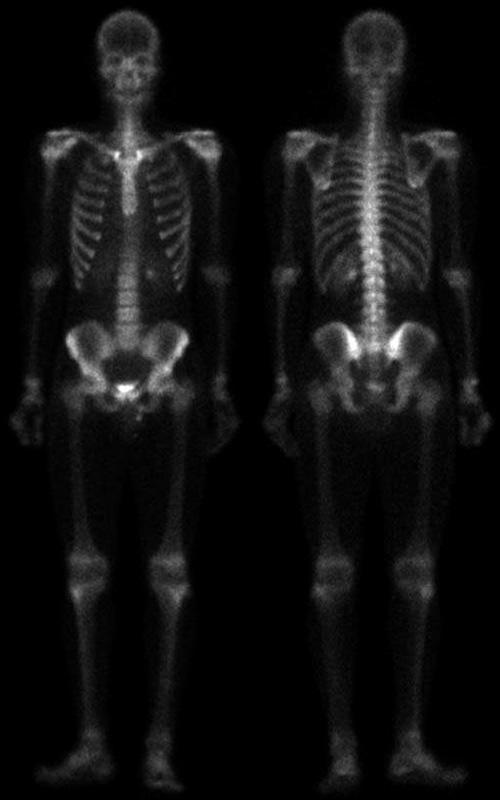
\includegraphics[width=0.25\textwidth]{../data/skeleton_orig.jpg}
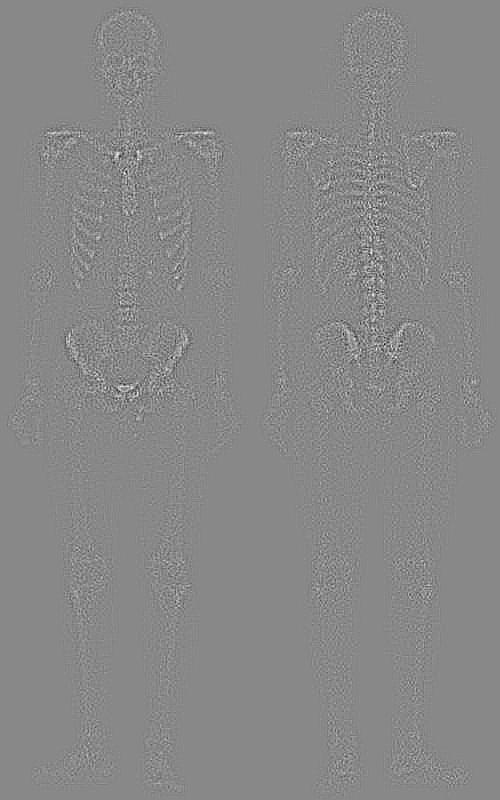
\includegraphics[width=0.25\textwidth]{../data/laplace_skeleton_orig.jpg}
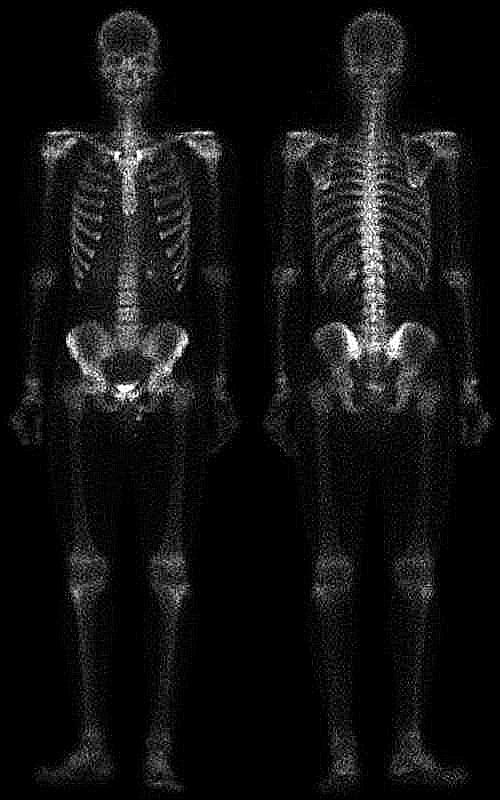
\includegraphics[width=0.25\textwidth]{../data/laplacian_skeleton_orig.jpg}
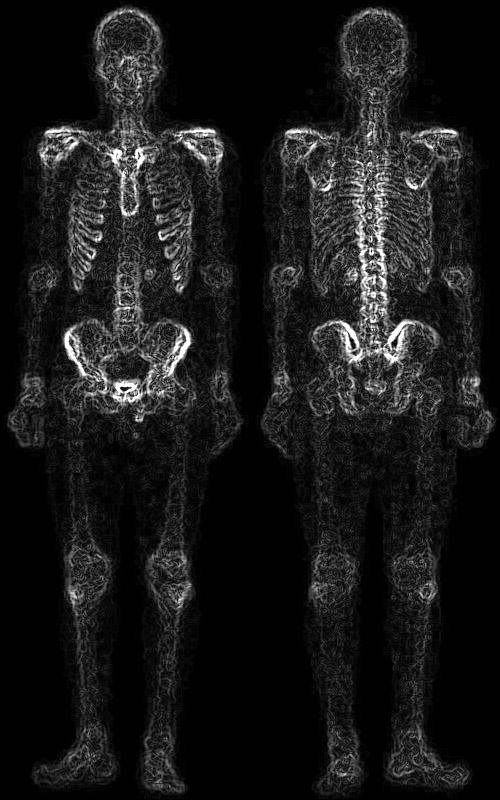
\includegraphics[width=0.25\textwidth]{../data/sobel_skeleton_orig.jpg}

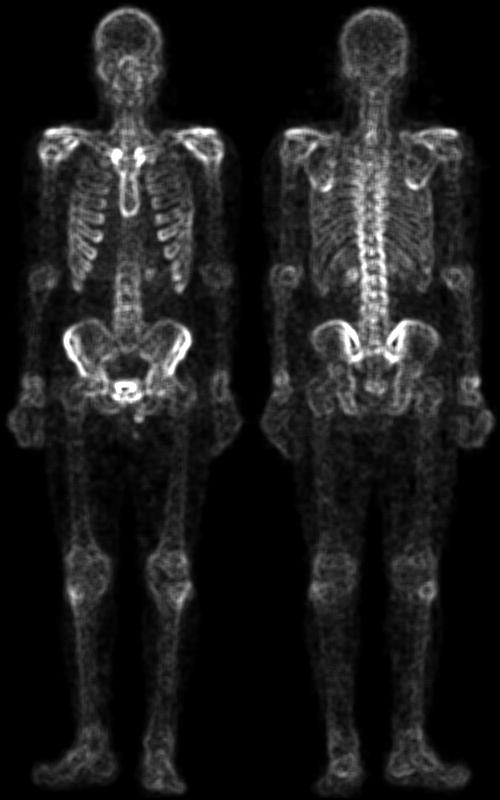
\includegraphics[width=0.25\textwidth]{../data/average_sobel_skeleton_orig.jpg}
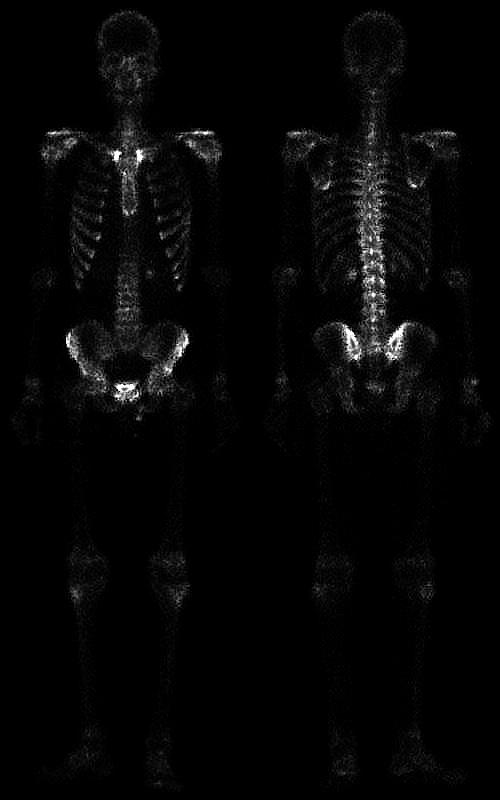
\includegraphics[width=0.25\textwidth]{../data/product_skeleton_orig.jpg}
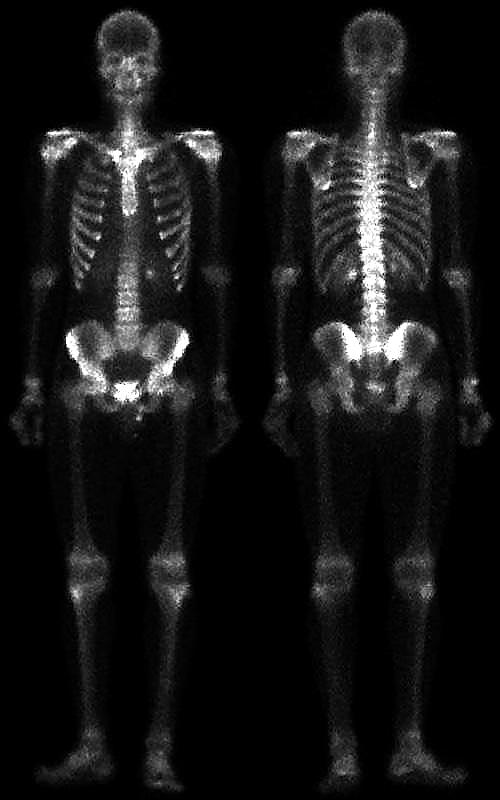
\includegraphics[width=0.25\textwidth]{../data/mix_skeleton_orig.jpg}
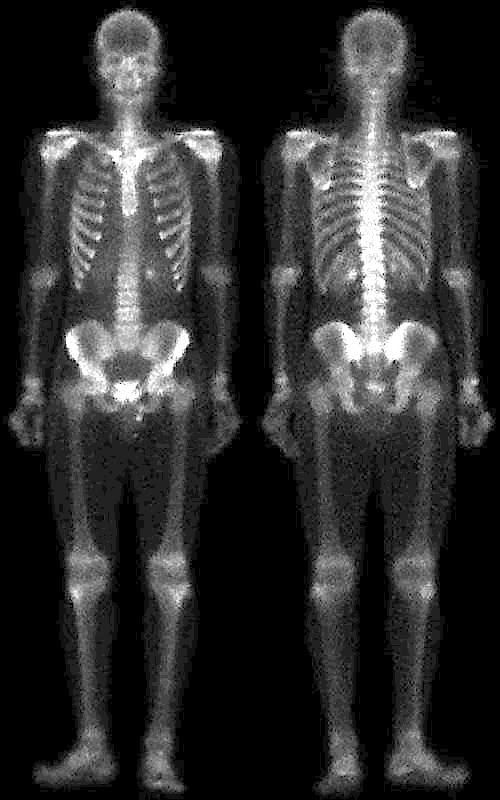
\includegraphics[width=0.25\textwidth]{../data/gamma_skeleton_orig.jpg}

\section{Laplacian Mask}
The Laplacian mask which we used is 
\begin{tabular}{|c|c|c|}
	\hline -1&-1&-1\\
	\hline -1&8&-1\\
	\hline -1&-1&-1\\
	\hline
\end{tabular}. 
The second is Laplacian image and the third one is the Laplacian filtered result. We can see the third image has more details but also has more noises than the first one.

\section{Sobel Gradient Mask}
To remove the noises in the third image, we use the Sobel gradient masks which are
\begin{tabular}{|c|c|c|}
	\hline -1&-2&-1\\
	\hline 0&0&0\\
	\hline 1&2&1\\
	\hline
\end{tabular} and 
\begin{tabular}{|c|c|c|}
	\hline -1&0&1\\
	\hline -2&0&2\\
	\hline -1&0&1\\
	\hline
\end{tabular}. 
The fourth image shows the result of Sobel gradient filter and then apply a $5\times5$ averaging mask to get the fifth image. We can see in these two figures, the edges are clearer. The sixth image is the product of the Laplacian result and the Sobel result. Add the product to the original image, we get a quite good result, the seventh image.

\section{Gamma Transformation}
The final step is to increase the active range of the gray level. We use gamma transformation $s=cr^\gamma$, here $c=1$ and $\gamma=0.5$. The result is the eighth image. Compare to the first image, we get more details without adding too many noises.

\end{document}